% Background: a GPU read of one page without the accessed flag. In a writable
% private mapping the fault is served as a write to the 2 MiB block and every
% page of the block becomes a private copy; in a read-only mapping the pages
% stay in place.
\documentclass[border=2pt]{standalone}
% Shared TikZ style of the STATOR design figures. Teal marks shared,
% immutable state; amber marks what one process writes; violet marks a
% second level of sharing; text is regular weight except the panel titles.
\usepackage{newtxtext}
\usepackage{tikz}
\usetikzlibrary{arrows.meta, positioning, fit, calc, patterns, shapes.geometric, decorations.pathreplacing}

\definecolor{panel}{HTML}{F3F4F6}   % a group of components
\definecolor{gpuc}{HTML}{E4E0F6}    % the GPU
\definecolor{ptc}{HTML}{FAF0DC}     % page tables and the SMMU
\definecolor{modelc}{HTML}{CDEBE6}  % the weights
\definecolor{sharedc}{HTML}{7FCBC1} % shared rows, read-only
\definecolor{tailc}{HTML}{F7B955}   % rows of one process, in use
\definecolor{aheadc}{HTML}{FCE6C2}  % populated ahead, or write-protected
\definecolor{copyc}{HTML}{F4BFCB}   % a copied page
\definecolor{segc}{HTML}{B7A9E8}    % the segment of a second ancestor
\definecolor{faultc}{HTML}{E8736A}  % a private copy made by a fault
\definecolor{actc}{HTML}{FDE9C9}    % an operation of the design
\definecolor{roline}{HTML}{14786F}  % read-only mappings
\definecolor{rwline}{HTML}{C5432F}  % writable mappings and faults

\tikzset{
  layer/.style={draw=black!60, fill=panel, line width=0.5pt},
  sub/.style={draw=black!55, line width=0.4pt},
  comp/.style={draw=black!85, fill=white, line width=0.4pt, align=center,
               font=\scriptsize, inner xsep=3pt, inner ysep=1.5pt, minimum height=0.5cm},
  seg/.style={draw=black!65, line width=0.35pt, inner sep=0pt, align=center,
              font=\scriptsize, minimum height=0.4cm},
  free/.style={seg, pattern=north east lines, pattern color=black!40},
  blk/.style={draw=black!65, line width=0.35pt, minimum width=0.42cm, minimum height=0.36cm,
              inner xsep=2pt, inner ysep=0pt, font=\scriptsize},
  hole/.style={blk, pattern=north east lines, pattern color=black!45},
  tag/.style={font=\scriptsize, inner sep=1pt},
  ttl/.style={font=\bfseries\small},
  lbl/.style={font=\scriptsize},
  note/.style={font=\itshape\scriptsize, inner sep=1pt},
  arr/.style={-{Latex[length=1.6mm]}, line width=0.8pt},
  thin/.style={-{Latex[length=1.3mm]}, line width=0.5pt},
  fat/.style={-{Triangle[length=2.2mm,width=3.4mm]}, line width=2.4pt},
  num/.style={circle, fill=black, text=white, font=\bfseries\scriptsize,
              inner sep=0.6pt, minimum size=0.33cm},
}
% A legend entry: a filled square and its name, at (x,y).
\newcommand{\legendfill}[4]{%
  \draw[black!65, line width=0.35pt, fill=#3] (#1,#2) rectangle ++(0.22,0.2);
  \node[tag, anchor=west] at (#1+0.27,#2+0.1) {#4};}
\newcommand{\legendhatch}[3]{%
  \draw[black!65, line width=0.35pt, pattern=north east lines, pattern color=black!45] (#1,#2) rectangle ++(0.22,0.2);
  \node[tag, anchor=west] at (#1+0.27,#2+0.1) {#3};}
% Legend marks for a legend that is one centred line of text:
%   \node[tag] at (x,y) {\lgdfill{sharedc}\,Shared \quad \lgdhatch\,Unbacked};
\newcommand{\lgdfill}[1]{\tikz[baseline=-0.55ex]{\draw[black!65, line width=0.35pt, fill=#1] (0,-0.1) rectangle (0.22,0.1);}}
\newcommand{\lgdhatch}{\tikz[baseline=-0.55ex]{\draw[black!65, line width=0.35pt, pattern=north east lines, pattern color=black!45] (0,-0.1) rectangle (0.22,0.1);}}

\begin{document}
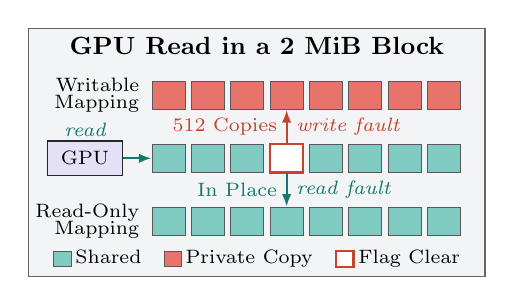
\begin{tikzpicture}[x=1cm, y=1cm]
\draw[layer] (0,0) rectangle (5.8,3.15);
\node[ttl] at (2.9,2.93) {GPU Read in a 2 MiB Block};
% the outcome in a writable private mapping: the whole block is copied
\node[tag, anchor=east, align=right] at (1.45,2.3) {Writable\\[-2pt]Mapping};
\foreach \k in {0,...,7} {
  \node[blk, fill=faultc] (c\k) at (1.78+\k*0.5,2.3) {};
}
% the pages of the file, one without the accessed flag
\node[comp, fill=gpuc, minimum width=0.95cm, minimum height=0.44cm] (gpu) at (0.72,1.5) {GPU};
\foreach \k in {0,...,7} {
  \node[blk, fill=sharedc] (b\k) at (1.78+\k*0.5,1.5) {};
}
\node[blk, fill=white, draw=rwline, line width=0.9pt] (flag) at (b3) {};
\draw[arr, roline] (gpu.east) -- (b0.west);
\node[note, text=roline, anchor=south] at (0.72,1.74) {read};
% the outcome in a read-only mapping: the pages stay shared
\node[tag, anchor=east, align=right] at (1.45,0.7) {Read-Only\\[-2pt]Mapping};
\foreach \k in {0,...,7} {
  \node[blk, fill=sharedc] (d\k) at (1.78+\k*0.5,0.7) {};
}
% the two faults
\draw[arr, rwline] (b3.north) -- (c3.south);
\node[note, text=rwline, anchor=west] at (3.36,1.9) {write fault};
\node[tag, text=rwline, anchor=east] at (3.2,1.9) {512 Copies};
\draw[arr, roline] (b3.south) -- (d3.north);
\node[note, text=roline, anchor=west] at (3.36,1.1) {read fault};
\node[tag, text=roline, anchor=east] at (3.2,1.1) {In Place};
% legend
\node[tag] at (2.9,0.22) {\lgdfill{sharedc}\,Shared\quad\lgdfill{faultc}\,Private Copy\quad\tikz[baseline=-0.55ex]{\draw[rwline, line width=0.9pt, fill=white] (0,-0.1) rectangle (0.22,0.1);}\,Flag Clear};
\end{tikzpicture}
\end{document}
